\PassOptionsToPackage{unicode}{hyperref}
\documentclass[t]{beamer}

\usepackage[
  orientation=portrait,
  size=a0,
  scale=1.0,
]{beamerposter}

\usetheme{tudoposter}

\usepackage{fontspec}

%\usepackage{polyglossia}
%\setmainlanguage{german}
\usepackage[english]{babel}

\usepackage{csquotes}
\usepackage{microtype}
\usepackage{mathtools}

\usepackage{blindtext}

\usepackage{multicol}
\setlength{\columnsep}{1em}

\usepackage{xfrac}

\usepackage{tikz}
\usetikzlibrary{shapes, arrows, backgrounds, fit, tikzmark, arrows.meta, calc, quotes, angles, decorations.pathmorphing}

\usepackage[center]{caption}

\usepackage{siunitx}

\usepackage[export]{adjustbox}

\usepackage{xcolor}
\usepackage{listings}
\lstset{
  commentstyle=\color{black!60},    % comment style
}

\lstdefinestyle{base}{
  moredelim=**[is][\color{black!30}]{@}{@},
}

\usepackage{mdframed} %nice frames
\definecolor{light-gray}{gray}{0.95} %the shade of grey that stack exchange uses

\definecolor{seaborn0}{HTML}{0072B2}
\definecolor{seaborn1}{HTML}{009E73}
\definecolor{seaborn2}{HTML}{D55E00}
\definecolor{seaborn3}{HTML}{CC79A7}
\definecolor{seaborn4}{HTML}{F0E442}
\definecolor{seaborn5}{HTML}{56B4E9}

\usepackage{graphicx}

% Evaluate at command
\NewDocumentCommand{\evalat}{sO{\big}mm}{%
  \IfBooleanTF{#1}
   {\mleft. #3 \mright|_{#4}}
   {#3#2|_{#4}}%
}


%% this is used to create an inline bibliography
\usepackage[backend=biber, style=numeric, sorting=none]{biblatex}
\addbibresource{biblatex-phys.bib}

\DeclareFieldFormat*{title}{\textit{#1}}
\renewcommand*{\bibfont}{\footnotesize}
\defbibenvironment{bibliography}
  {\noindent}
  {\unspace}
  {}

\renewbibmacro*{begentry}{%
  \usebeamercolor{bibliography item}%
  \color{bibliography item.fg}%
  \printtext[labelnumberwidth]{%
    \printfield{prefixnumber}%
    \printfield{labelnumber}%
  }%
  \setunit{\addnbspace}%
}
\renewcommand*{\finentrypunct}{\addperiod\space}

\newlength{\thirdtextwidth}
\setlength\thirdtextwidth{0.333333\textwidth}

\newlength{\itemseparation}
\setlength\itemseparation{0.25em}

\title{Physics updates of the high-energy lepton and photon simulation tool PROPOSAL}
\author{Jean-Marco Alameddine$^{1}$, Pascal Gutjahr$^{1}$, Wolfgang Rhode$^{1}$, Alexander Sandrock$^{2}$, \\Jan Soedingrekso$^{1}$}
\institute[ETH]{$^{1}$TU Dortmund University, Otto-Hahn-Str. 4a, 44227 Dortmund, Germany \\$^{2}$University of Wuppertal, Gaußstraße 20, 42119 Wuppertal, Germany}
\date{4. Juli 2015}

\titlegraphic{%
  
\includegraphics[width=1.2\linewidth, left]{images/tudo.pdf}\\
  \vspace{0.2em}
  
\includegraphics[width=0.95\linewidth, left]{images/BUW.png}\\
  %\vspace{0.2em}
  %\includegraphics[width=1.0\linewidth, left]{dfg_logo_englisch_blau_en.jpg}
}

%% underline 

\newcommand{\udot}[2]{%
    \tikz[baseline=(#2.base)]{
        \node[inner sep=1pt,outer sep=0pt] (#2) {#1};
        \draw[line width=0.2cm, tugreen] ($(#2.south west) - (0, 0.1)$) -- ($(#2.south east) - (0, 0.1)$);
    }%
}%

\begin{document}


  \begin{columns}[onlytextwidth]%
    \begin{column}{0.6\textwidth}%
      \begin{block}[equal height group=A]{Introduction}%
      \hspace{0.5cm}
      \begin{tikzpicture}
        \newfontfamily{\Chalkduster}{Chalkduster}
        \node [anchor=west, align=center, font=\Large] (title) at (0,0) {\udot{{\huge\textbf{PR}}opagator}{udot1} with \udot{{\huge\textbf{O}}ptimal {\huge\textbf{P}}recision and {\huge\textbf{O}}ptimized {\huge\textbf{S}}peed}{udot2} for \udot{{\huge\textbf{A}}ll {\huge\textbf{L}}eptons}{udot3}};        

        \node[text=red, rotate=10, font=\large, opacity=1.0] (A) at (41,-1.25) {\Chalkduster and photons};

        \node [anchor=west, align=center] (noteA) at (1, -3.4) {3D Monte Carlo simulation of \\individual particles \cite{koehne2013proposal, dunsch_2018_proposal_improvements}};

        \node [anchor=west, align=center] (noteB) at (15, -3.4) {Optimized for large-scale \\particle propagation};

        \node [anchor=west, align=center] (noteC) at (27, -3.4) {Simulations of high-energy electrons, \\positrons, photons, muons, and taus};

        \draw[-latex, line width=4pt, tugreen] (4, -0.8) -- ($(noteA.north) - (0.5, 0)$);

        \draw[-latex, line width=4pt, tugreen] (21, -0.8) -- ($(noteB.north) - (0, 0)$);

        \draw[-latex, line width=4pt, tugreen] (37, -0.8) -- ($(noteC.north) - (0, 0)$);


        %\draw [-latex, line width=4pt, tugreen] (udot1.south) to[out=-45, in=125] (noteA.north);

        %\draw [-latex, line width=4pt, tugreen] (udot2.south) to[out=-45, in=125] (noteB.north);

        %\draw [-latex, line width=4pt, tugreen] (udot3) to[out=-45, in=125] (noteC.north);



        %\begin{scope}[xshift=1.5cm]
        %  \node[anchor=south west,inner sep=0] (image) at (0,0) {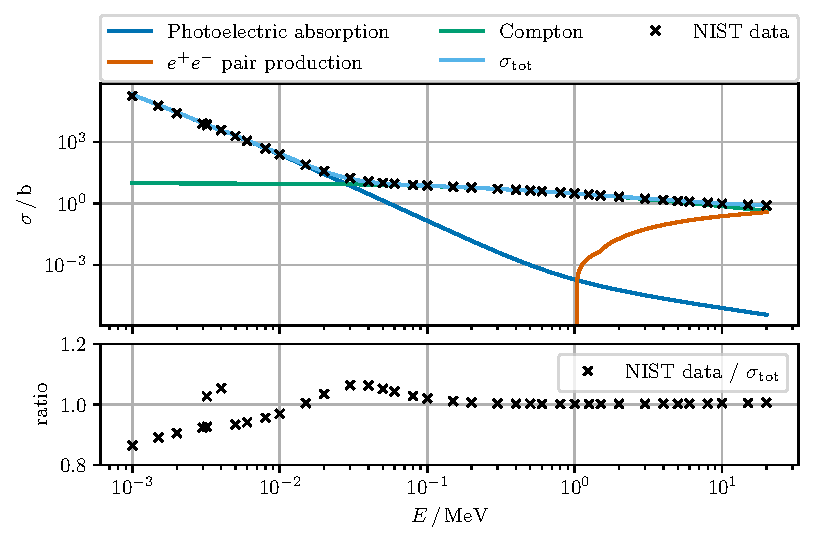
\includegraphics[width=0.6\textwidth]{../plots/photoeffect_nist.pdf}};
        %  \begin{scope}[x={(image.south east)},y={(image.north west)}]
        %      \draw[tugreen,line width=4pt,rounded corners] (0.24,0.17) rectangle ++(0.041,0.15); % point to resonances
        %      \draw [-latex, line width=4pt, tugreen] (noteA) to[out=-45, in=-90] (0.2605,0.165);
        %      \draw[tugreen,line width=4pt,rounded corners] (0.15,0.70) rectangle ++(0.21,0.14); % point to very-low energy regime
        %      \draw [-latex, line width=4pt, tugreen] (noteB) to[out=45, in=180] (0.145,0.77);
        %      \draw[tugreen,line width=4pt,rounded corners] (0.70,0.6) rectangle ++(0.25,0.07); % point to high-energy regime
        %      \draw [-latex, line width=4pt, tugreen] (noteC) to[out=90, in=45] (0.95,0.67);
        %  \end{scope}
        %\end{scope}
      \end{tikzpicture}%


      \end{block}
    \end{column}
    \begin{column}{0.4\textwidth}%
      \begin{block}[equal height group=A]{Installation}%
        \begin{columns}[onlytextwidth]
          \begin{column}{0.7\textwidth}%
            \textbf{PROPOSAL is a C\texttt{++}14 library with Python bindings}
            \begin{itemize}
              \setlength\itemsep{\itemseparation}
              \item[$\rightarrow$] Simple Python installation with \colorbox{tuYellow}{\texttt{pip install proposal}}
              \item[$\rightarrow$] C\texttt{++} installation via CMake, or with the package manager Conan
            \end{itemize}
          \end{column}
          \begin{column}{0.3\textwidth}%
            \vspace{-1.3cm}
            \begin{figure}
              
\includegraphics[width=0.75\linewidth, keepaspectratio]{images/cpp-python.png}
            \end{figure}
          \end{column}
        \end{columns}
      \end{block}
    \end{column}
    \end{columns}





  \begin{columns}[onlytextwidth]%
    \begin{column}{\textwidth}%
      \begin{block}{Physics improvements for photon interactions}%
        \vspace{0.6cm}
        \begin{minipage}[t]{0.3\textwidth}
          \begin{minipage}[t][11cm]{\textwidth}
            {\Large\textbf{Photoelectric absorption:}}
            \begin{columns}[onlytextwidth]
                \begin{column}{0.6\textwidth}%
                  \begin{itemize}[leftmargin=0.5cm]
                    \item Dominant interaction type for photon energies below $\approx \SI{30}{\kilo\electronvolt}$
                    \item Accurate description complicated, but not necessary for development of electromagnetic cascades
                    \begin{itemize}
                      \item[$\rightarrow$] Implementation of an approximate description
                    \end{itemize}
                  \end{itemize}
                \end{column}
                \begin{column}{0.35\textwidth}%
                  \vspace{0.5cm}
                  \begin{figure}
                    \begin{tikzpicture}[>=stealth', pos=.55, photon/.style={decorate,decoration={snake,post length=2mm}}]
                      \draw[draw=seaborn0, fill=seaborn0, fill opacity=0.2, line width=0.2cm] (0, 0) rectangle ++(6.5,1.8);
                      \draw[->,photon, line width=0.05cm] (0,4) -- node[above] {$\gamma$} (2.95, 1.3);

                      \draw[->, line width=0.05cm] (3.55, 1.35) -- node[above] {} (5.75, 3.6);


                      \node[circle,draw=darkgray, fill opacity=1.0,line width=0.05cm,inner sep=0mm, minimum size=0.85cm] (c) at (0.85,0.9){\footnotesize$e^-$};
                      \node[circle,draw=darkgray, fill opacity=1.0,line width=0.05cm,inner sep=0mm, minimum size=0.85cm] (c) at (2.05,0.9){\footnotesize$e^-$};

                      \node[circle,draw=darkgray, fill opacity=0.5, draw opacity=0.5, line width=0.05cm,inner sep=0mm, minimum size=0.85cm] (c) at (3.25,0.9){\footnotesize$e^-$};                      
                      \node[circle,draw=darkgray, fill opacity=1.0,line width=0.05cm,inner sep=0mm, minimum size=0.85cm] (c) at (4.45,0.9){\footnotesize$e^-$}; 
                      \node[circle,draw=darkgray, fill opacity=1.0,line width=0.05cm,inner sep=0mm, minimum size=0.85cm] (c) at (5.65,0.9){\footnotesize$e^-$}; 

                      \node[circle,draw=darkgray, fill opacity=1.0,line width=0.05cm,inner sep=0mm, minimum size=0.85cm] (c) at (6.2,4.1){\footnotesize$e^-$};

                    \end{tikzpicture}
                      %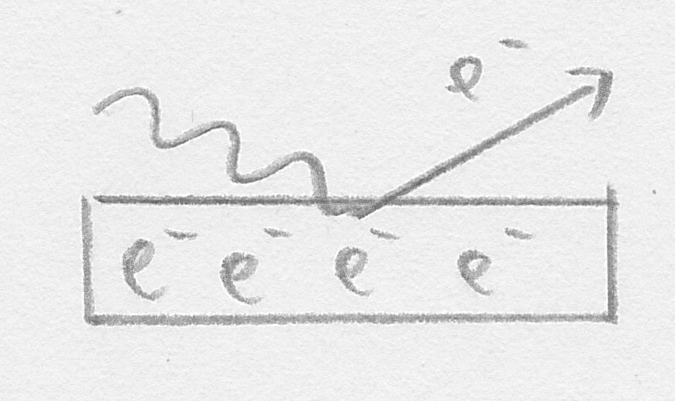
\includegraphics[width=\linewidth, keepaspectratio]{images/photoeffect_sketch.png}
                    \end{figure}
                \end{column}
            \end{columns}     
            %\begin{itemize}[itemindent=0.85cm,topsep=0.22cm,leftmargin=0.5cm]
            %          \item[$\rightarrow$] Agrees within \SI{10}{\percent} with NIST data
            %\end{itemize}     
          \end{minipage}
          \begin{minipage}[t][10cm]{\textwidth}
           {\Large\textbf{LPM effect:}}
            \begin{columns}[onlytextwidth]
                \begin{column}{0.6\textwidth}%
                  \begin{itemize}[leftmargin=0.5cm]
                    \item Suppression of small bremsstrahlung losses and symmetric pair production processes
                    \item Relevant for high energies and/or dense media
                  \end{itemize}
                \end{column}            
                \begin{column}{0.35\textwidth}%
                  \begin{figure}
                    \begin{tikzpicture}[>=stealth', pos=.35, photon/.style={decorate,decoration={snake,post length=2mm}}]
                      
                      % formation zone
                      \draw [draw=seaborn2, fill=seaborn2, fill opacity=0.2, line width=0.1cm] (3.5,0) ellipse (1.8cm and 0.8cm);
                      \node[text=seaborn2, align=center, font=\footnotesize] at (3.5,-1.6) {formation \\length};
                      %photon
                      \draw[->,photon, line width=0.05cm] (0,0) -- node[above] {$\gamma$} (3, 0);
                      
                      %electron
                      %\draw[->, line width=0.05cm, draw opacity=0.5] (3.2,0) -- node[text=seaborn2, above] {$e^-$} (7, 1.5);
                      \draw[->, line width=0.05cm, pos=0.75] (3.2,0) -- (3.4, 0.05) -- (3.6, 0.2) -- (3.8, 0.21) -- (4.0, 0.35) -- (4.2, 0.39) -- node[text=black, above] {$e^-$} (7, 1.5);

                      %positron
                      %\draw[->, line width=0.05cm, draw opacity=0.5] (3.2,0) -- node[text=seaborn2, below] {} (7, -1.5);
                      \draw[->, line width=0.05cm, pos=0.75] (3.2,0) -- (3.4, -0.1) -- (3.6, -0.1) -- (3.8, -0.28) -- (4.0, -0.27) -- (4.2, -0.39) -- node[text=black, below] {$e^+$} (7, -1.5);


                    \end{tikzpicture}
                    %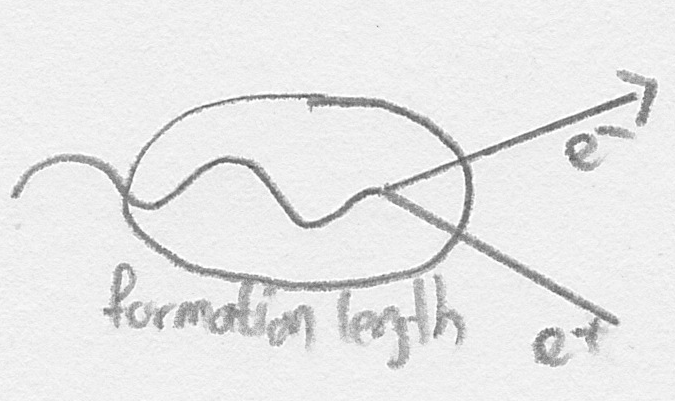
\includegraphics[width=\linewidth, keepaspectratio]{images/lpm_sketch.png}
                    \end{figure}
                \end{column}            
            \end{columns}
          \end{minipage}
        \end{minipage}
        \begin{minipage}[t]{0.4\textwidth}
          \begin{figure}
            \vspace{1cm}
            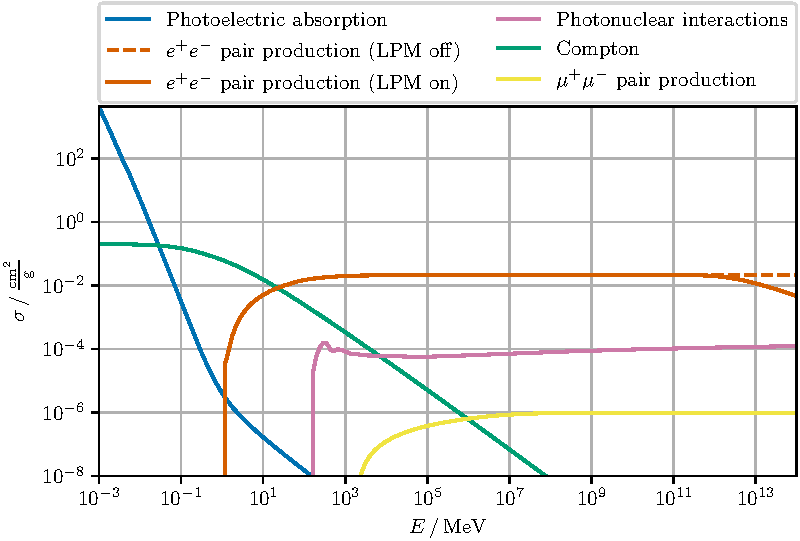
\includegraphics[width=0.9\linewidth, keepaspectratio]{../plots/Photon_Air_dndx_ecut_0.pdf}
          \end{figure}
        \end{minipage}
        \begin{minipage}[t]{0.3\textwidth}
          \begin{minipage}[t][11cm]{\textwidth}
             {\Large\textbf{Photonuclear interactions:}}
            \begin{columns}[onlytextwidth]
                \begin{column}{0.35\textwidth}%
                  \vspace{1.0cm}
                  \begin{figure}
                    \begin{tikzpicture}[>=stealth', pos=.55, photon/.style={decorate,decoration={snake,post length=2mm}}]

                      \path (-2,-2) rectangle (2,2);
                      \pgfmathdeclarerandomlist{color}{{seaborn4}{white}}
                      \pgfmathsetseed{2}
                      \foreach \A/\R in {20/0.7,12/0.5,7/0.3,1/0}{
                            \pgfmathsetmacro{\S}{360/\A}
                                 \foreach \B in {0,\S,...,360}{
                                     \pgfmathrandomitem{\C}{color}
                                     \shade[ball color=\C] (\B+\A:\R) circle (5pt);
                                 }
                      }

                      \draw[->,photon, line width=0.05cm] (-4.0,0) -- node[above] {$\gamma$} (-1.1, 0);
                      \draw[->, line width=0.05cm] (1.2,0.3) -- node[above] {} (3.8, 0.8);
                      \draw[->, line width=0.05cm] (1.2,0.) -- node[above] {} (3.9, 0.2);
                      \draw[->, line width=0.05cm] (1.2,-0.38) -- node[above] {} (3.85, -0.58);
                      \node[text=black, align=center, font=\footnotesize] at (2.4,-1.1) {Hadrons};

                      %\draw[->, line width=0.05cm] (3.2,0) -- node[text=seaborn4, above] {$\mu^-$} (7, 1.5);
                      %\draw[->, line width=0.05cm] (3.2,0) -- node[text=seaborn4, below] {$\mu^+$} (7, -1.5);

                    \end{tikzpicture}
                      %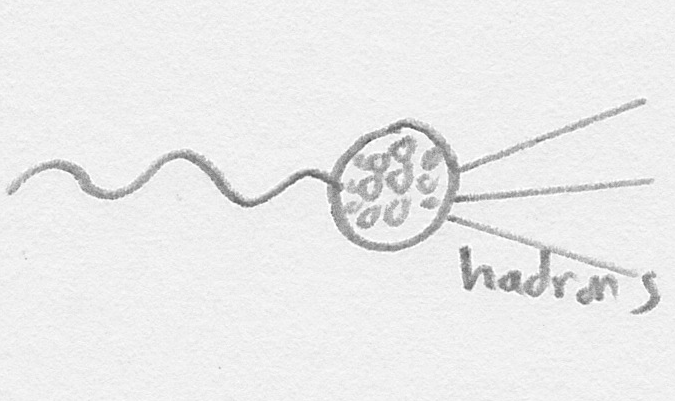
\includegraphics[width=\linewidth, keepaspectratio]{images/photoproduction_sketch.png}
                    \end{figure}
                \end{column}
                \begin{column}{0.6\textwidth}%
                  \begin{itemize}[leftmargin=0.5cm]
                    \item Absorption of photon by nucleus
                    \item Source of hadrons (and consequently muons) from electromagnetic cascades
                    \item Extrapolation to high energies has high uncertainties
                    \begin{itemize}
                      \item[$\rightarrow$] Different parametrizations available
                    \end{itemize}
                  \end{itemize}
                \end{column}                
            \end{columns}    
          \end{minipage}
          \begin{minipage}[t][10cm]{\textwidth}
            {\Large\textbf{Muon pair production:}}
            \begin{columns}[onlytextwidth]
                \begin{column}{0.35\textwidth}%
                  \begin{figure}
                    \begin{tikzpicture}[>=stealth', pos=.55, photon/.style={decorate,decoration={snake,post length=2mm}}]
                      \draw[->,photon, line width=0.05cm] (0,0) -- node[above] {$\gamma$} (3, 0);
                      \draw[->, line width=0.05cm] (3.2,0) -- node[text=seaborn3, above] {$\mu^-$} (7, 1.5);
                      \draw[->, line width=0.05cm] (3.2,0) -- node[text=seaborn3, below] {$\mu^+$} (7, -1.5);

                    \end{tikzpicture}
                      %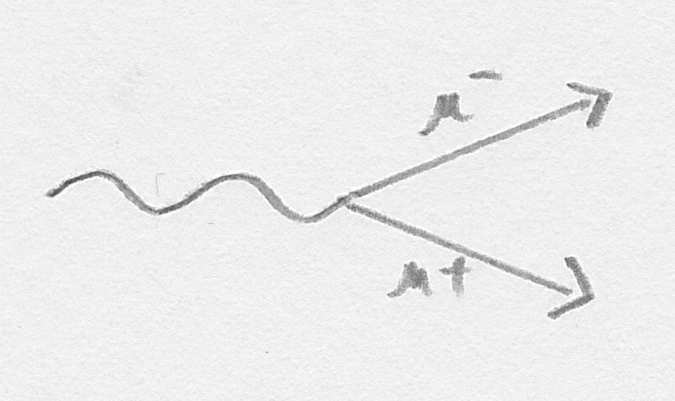
\includegraphics[width=\linewidth, keepaspectratio]{images/mupair_sketch.png}
                    \end{figure}
                \end{column}            
                \begin{column}{0.6\textwidth}%
                  \begin{itemize}[leftmargin=0.5cm]
                    \item Subdominant process compared to $e^- e^+$ pair production
                    \item Source of muons from electromagnetic cascades

                  \end{itemize}
                \end{column}
            \end{columns}
          \end{minipage}
        \end{minipage}

      \end{block}
    \end{column}
    \end{columns}


  \begin{columns}[onlytextwidth]%
    \begin{column}{0.55\textwidth}%
      \begin{block}[equal height group=PLOTS]{Validation of low-energy photon cross sections}%

      \textbf{Comparison of PROPOSAL implementation to calculations from NIST Standard Reference Database \cite{nist}}

      \vspace{0.5cm}

      \begin{tikzpicture}
        \centering
        \node [anchor=west, align=center] (noteA) at (-7.5,4) {Expected discrepancies \\around absorption lines\\ (here: K-line of \textup{Ar})};
        \node [anchor=west, align=center] (noteB) at (-7.5, 12) {Agreement better than \\\SI{10}{\percent} even at low \\energies where used \\parametrization is not \\expected to be exact };        
        \node [anchor=west, align=center] (noteC) at (+27, 8) {Good agreement \\for energies where\\ pair production and\\ Compton are \\dominant processes};        


        \begin{scope}[xshift=1.5cm]
          \node[anchor=south west,inner sep=0] (image) at (0,0) {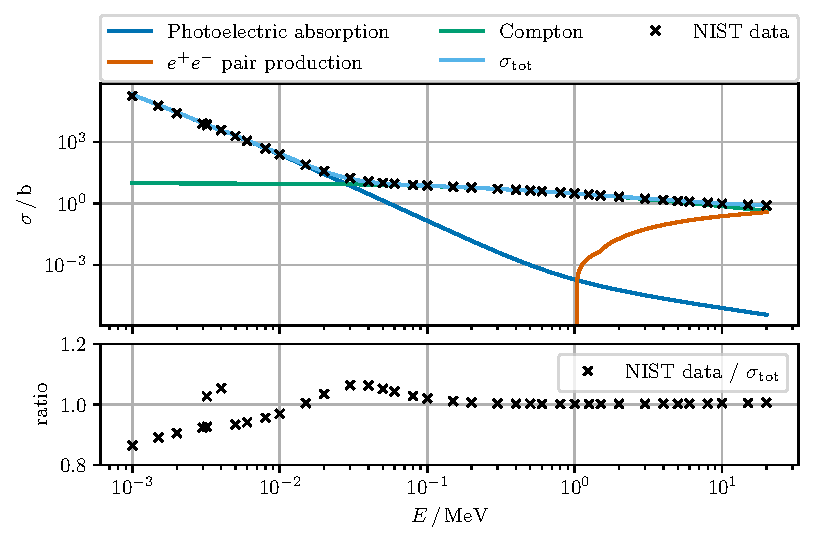
\includegraphics[width=0.6\textwidth]{../plots/photoeffect_nist.pdf}};
          \begin{scope}[x={(image.south east)},y={(image.north west)}]
              \draw[tugreen,line width=4pt,rounded corners] (0.24,0.17) rectangle ++(0.041,0.15); % point to resonances
              \draw [-latex, line width=4pt, tugreen] (noteA) to[out=-45, in=-90] (0.2605,0.165);

              \draw[tugreen,line width=4pt,rounded corners] (0.15,0.70) rectangle ++(0.21,0.14); % point to very-low energy regime
              \draw [-latex, line width=4pt, tugreen] (noteB) to[out=45, in=180] (0.145,0.77);

              \draw[tugreen,line width=4pt,rounded corners] (0.70,0.6) rectangle ++(0.25,0.07); % point to high-energy regime
              \draw [-latex, line width=4pt, tugreen] (noteC) to[out=90, in=45] (0.95,0.67);

          \end{scope}
        \end{scope}
      \end{tikzpicture}%

              %\begin{figure}
              %    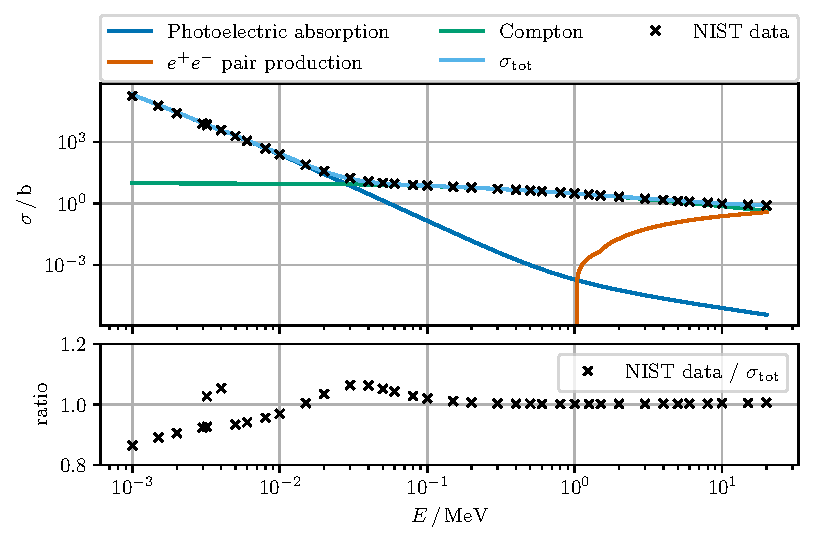
\includegraphics[width=0.7\linewidth, keepaspectratio]{../plots/photoeffect_nist.pdf}
              %  \end{figure}
      \end{block}
    \end{column}
    \begin{column}{0.45\textwidth}%
      \begin{block}[equal height group=PLOTS]{Impact of LPM effect on air showers}%

      \textbf{Influence of the LPM effect on pair production processes in air}

      \vspace{0.0cm}

              \begin{figure}
              \begin{minipage}[t]{0.49\textwidth}
                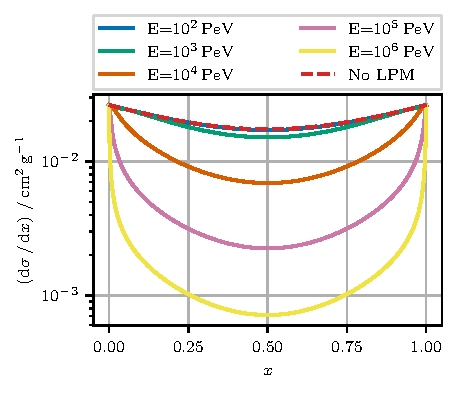
\includegraphics[width=\linewidth, keepaspectratio]{../plots/lpm_photopair_differential_small.pdf}
                \vspace{-1.5cm}
                \begin{itemize}
                  \item For air at sea level, suppression of symmetric pair production processes at energies above \SI{e2}{\peta\electronvolt}

                \end{itemize}
              \end{minipage}%
              \hfill
              \begin{minipage}[t]{0.49\textwidth}
                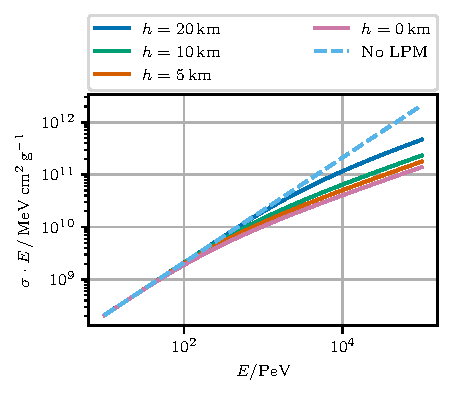
\includegraphics[width=\linewidth, keepaspectratio]{../plots/lpm_cross_photopair_small.pdf}
                  \vspace{-1.5cm}
                  \begin{itemize}
                      \item LPM suppression is density dependent, and therefore dependent on height in atmosphere
                  \end{itemize}
              \end{minipage}
              \end{figure}
      \end{block}
    \end{column}
    \end{columns}



  \begin{columns}[onlytextwidth]%
    \begin{column}{0.55\textwidth}%
      \begin{block}[equal height group=F]{How to use PROPOSAL}%
        \vspace{-0.75em}
        \begin{columns}[onlytextwidth]
        \begin{column}{0.48\textwidth}

        \begin{tikzpicture}
          \centering
          \node [anchor=west, align=center, font=\small] (noteA) at (14.5,13) { Information about environment \\in json configuration file};     

          \begin{scope}[xshift=1.5cm]
              \node[anchor=south west,inner sep=0] (image) at (0,0) {

              \lstinputlisting[
              language=Python,
              basicstyle=\footnotesize\ttfamily,
              style=base,
              escapechar=\$,
              breaklines=true
              ]{code/example.txt}
            };
            \begin{scope}[on background layer]
              \draw[draw=light-gray, fill=light-gray] ($(image.south east)+(0.4, -0.4)$) rectangle ($(image.north west)+(-0.4, 0)$);
            \end{scope}
            \begin{scope}[x={(image.south east)},y={(image.north west)}]
              %\draw[tugreen,line width=4pt,rounded corners] (0.24,0.17) rectangle ++(0.041,0.15); % point to resonances
              \draw [-latex, line width=4pt, tugreen] (noteA) to[out=-125, in=60] (0.71, 0.75);

              %\draw[tugreen,line width=4pt,rounded corners] (0.15,0.70) rectangle ++(0.21,0.14); % point to very-low energy regime
              %\draw [-latex, line width=4pt, tugreen] (noteB) to[out=45, in=180] (0.145,0.77);

              %\draw[tugreen,line width=4pt,rounded corners] (0.70,0.6) rectangle ++(0.25,0.07); % point to high-energy regime
              %\draw [-latex, line width=4pt, tugreen] (noteC) to[out=90, in=45] (0.95,0.67);
            \end{scope}
          \end{scope}
        \end{tikzpicture}%
 
          \end{column}
          \begin{column}{0.07\textwidth}
          \begin{center}
            \vspace{7.5em}
            \begin{tikzpicture}
            \draw[
              -triangle 90,
               line width=4mm,
                postaction={draw, line width=0.7cm, shorten >=1cm, -}
            ] (0,0) -- (2,0);
          \end{tikzpicture}
          \end{center}          
        \end{column}
          \begin{column}{0.45\textwidth}
            \vspace{-1.0cm}
            \begin{figure}
              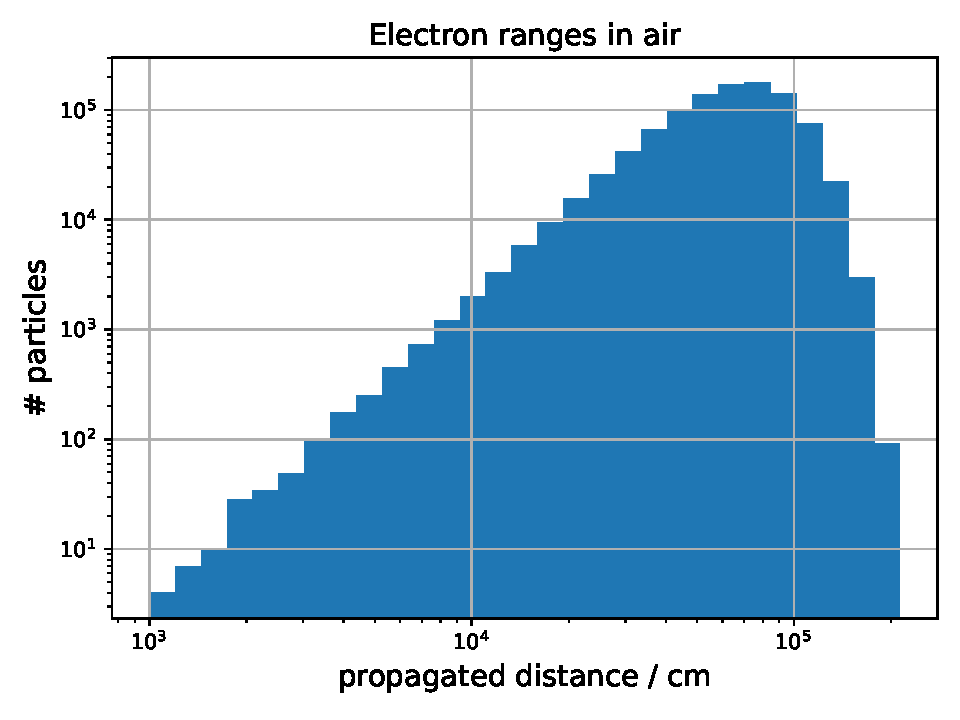
\includegraphics[width=\linewidth, height=.4\textheight, keepaspectratio]{code/example_output.pdf}
            \end{figure}
          \end{column}
        \end{columns}
 
      \end{block}%
    \end{column}%
    \begin{column}{0.45\textwidth}%
      \begin{block}[equal height group=F, left=-5mm, right=-5mm, lefttitle=4mm, top=-5mm, bottom=-5mm]{Application: CORSIKA 8}%
        \begin{tikzpicture}[path image/.style={path picture={
                   \node at ($(path picture bounding box.center)+(0.5,0)$) {
                            \includegraphics[scale=0.75, rotate=-63]{#1}};}
                   }]
        \centering
        \node [anchor=west, align=center] (noteA) at (2.5,12.3) {PROPOSAL is used to simulate the \\electromagnetic and muonic shower \\component in the new particle-shower\\ simulation code CORSIKA~8 \cite{Engel2018}};
        \node [anchor=west, align=center] (noteA) at (14.1,2.5) {$\rightarrow$ For more details, see talks by A.~Sandrock [CRI19-06]\\ and T.~Huege [CRI20-08] on Wednesday};
        %\node [anchor=west, align=center] (noteB) at (-7.5, 12) {Agreement better than \\\SI{10}{\percent} even at low \\energies where used \\parametrization is not \\expected to be exact };        
        %\node [anchor=west, align=center] (noteC) at (+27, 8) {Good agreement \\for energies where\\ pair production and\\ Compton are \\dominant processes};        
        \begin{scope}[on background layer]
              \path [path image=images/shower_raw_2.png, opacity=0.8] (0,0) rectangle (\linewidth, 16.2cm);
        \end{scope}

              


        \begin{scope}
          % REPLACE WITH REAL png
          %\node[anchor=south west,inner sep=0] (image) at (0,0) {\includegraphics[width=0.6\textwidth, rotate=-45]{images/shower_raw_2_draft.jpeg}};
          \begin{scope}[x={(image.south east)},y={(image.north west)}]
              %\draw[tugreen,line width=4pt,rounded corners] (0.24,0.17) rectangle ++(0.041,0.15); % point to resonances
              %\draw [-latex, line width=4pt, tugreen] (noteA) to[out=-45, in=-90] (0.2605,0.165);

              %\draw[tugreen,line width=4pt,rounded corners] (0.15,0.70) rectangle ++(0.21,0.14); % point to very-low energy regime
              %\draw [-latex, line width=4pt, tugreen] (noteB) to[out=45, in=180] (0.145,0.77);

              %\draw[tugreen,line width=4pt,rounded corners] (0.70,0.6) rectangle ++(0.25,0.07); % point to high-energy regime
              %\draw [-latex, line width=4pt, tugreen] (noteC) to[out=90, in=45] (0.95,0.67);
          \end{scope}
        \end{scope}
        \end{tikzpicture}%
      \end{block}%
    \end{column}%    
    \end{columns}



  \begin{columns}[onlytextwidth]%
    \begin{column}{0.4\textwidth}%
      \begin{block}[equal height group=Z]{Summary}%
        \begin{itemize}
          \item Implementation of new photon processes relevant at low and high energies
          \begin{itemize}
            \item[$\rightarrow$] Complete description of electrons, positrons, and photons in the regime relevant for electromagnetic cascades
          \end{itemize}
          \item PROPOSAL is a highly flexible framework for lepton and photon simulations
        \end{itemize}
      \end{block}
    \end{column}
    \begin{column}{0.4\textwidth}%
      \begin{block}[equal height group=Z]{Contact}%
        \begin{center}
          \begin{figure}[ht]
            \begin{minipage}[ht]{0.75\linewidth}
              \textbf{Find the PROPOSAL repository under:}\\ \url{github.com/tudo-astroparticlephysics/PROPOSAL} \vspace{0.5em}\\
              \textbf{Contact via mail:}\\ \href{mailto:me@jean-marco.alameddine@tu-dortmund.de}{jean-marco.alameddine@tu-dortmund.de} 
            \end{minipage}
            \begin{minipage}[ht]{0.24\linewidth}
              \centering
                
\includegraphics[width=0.66\linewidth, valign=t]{images/qr_proposal.png}
            \end{minipage}
          \end{figure}
        \end{center}
      \end{block}
    \end{column}
    \end{columns}

  \vspace*{\fill}
  \begin{columns}[onlytextwidth]%
    \begin{column}{0.75\textwidth}%
      \begin{alertblock}[equal height group=bottom, fonttitle=\normalsize]{References}
        \begin{multicols}{3}
          \footnotesize%
          \printbibliography%
        \end{multicols}
      \end{alertblock}
    \end{column}
    \begin{column}{0.25\textwidth}%
      \begin{alertblock}[equal height group=bottom, fonttitle=\normalsize]{Acknowledgments}
          \footnotesize%
          This work has been supported by the Deutsche Forschungsgemeinschaft (DFG) and the Lamarr institute.
          Jean-Marco Alameddine acknowledges the financial support by the German Academic Exchange Service (DAAD).
      \end{alertblock}
    \end{column}
  \end{columns}

  %\begin{block}[equal height group=bottom, fonttitle=\normalsize]{References}
  %  \begin{multicols}{3}
  %    \footnotesize%
  %    \printbibliography%
  %  \end{multicols}
  %\end{block}
\end{document}
